\documentclass{article}
\usepackage[top=1in,bottom=1in,left=1in,right=1in]{geometry}
\usepackage{listings}
\usepackage{hyperref}
\usepackage{color}
\usepackage[pdftex]{graphicx}
\usepackage{xspace}


\title{Models of FMDV in a Herd of Cattle}
\author{Drew Dolgert}
\date{\today}

\begin{document}
\maketitle
\abstract{There is significant data on the progress of FMDV within individual
cattle. This data describes both the progress of the disease and its variability
among individuals according to various effects. Obtaining multiple samples of
similar data for herds of infected cattle is impractical or inhumane, so
models extend understanding at an individual level to a herd level. This article
examines a family of models for FMDV progress within a herd in order to
understand how both the average progress of disease and an estimate of its
variability.}

\section{Introduction}
Focus on a putative herd of beef cattle of the same breed and similar life stage.
Build several models of varying complexity.


\section{FMDV progress within an individual}
\begin{figure}
\centerline{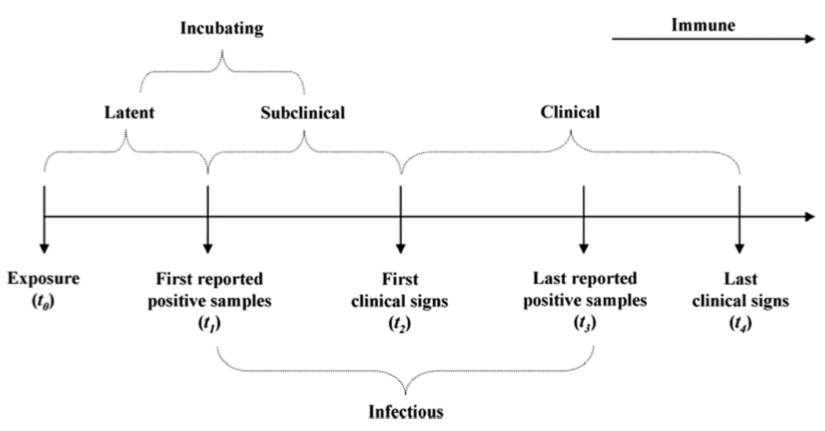
\includegraphics[width=9cm]{mardones_states}}
\caption{States of FMDV from Mardones et al.\cite{Mardones2010}.\label{fig:mardones_states}}
\end{figure}
\begin{figure}
\centerline{\begin{tabular}{llll}
\hline
FMD stage & time interval [days] & Poisson & Distribution \\ \hline
Latent &  $t_1-t_0$ & 3.59 & Weibull ($\alpha=1.782$, $\beta=3.974$) \\
Subclinical & $t_2-t_1$ & 2.04 & Gamma ($\alpha=1.222$, $\beta=1.672$) \\
Incubation & $t_2-t_0$  & 5.9 & Log logistic ($\gamma=0$, $\beta=5.3$, $\alpha=4.02$) \\
Infectious &  $t_3-t_1$ & 4.39 & Gamma ($\alpha=3.969$, $\beta=1.107$)
\end{tabular}}
\caption{From ``FMDV serotype O infection in domestic animals,''\label{fig:compartments}}
\end{figure}%
In an epidemiological context, the pathology of FMDV within an
individual is reduced to calculations of the rate of transitions
among compartmental states, each of which directly affects how
the individual interacts with the outside world. Each compartment
is defined on a condition that the pathology of the individual
cross some threshold. It reduces the individual to a statistical
observation of only the relevant effects of disease.

In a review paper,
Mardones et al.\ define five observation points for the progress of FMDV within
an individual, exposure at $t_0$, first reported positive sample
at $t_1$, first clinical sign at $t_2$, last reported positive sample at $t_3$,
and last clinical sign at $t_4$. These observations are the boundaries
of compartments for the FMDV compartmental model, as described
in Fig.~\ref{fig:compartments}.
The statistical sampling that defines the rate of transition
from one compartment to the next averages over individual
traits, such as route of infection, initial viral load,
and individual immune response, but the paper makes clear
how much variation is possible due to these causes.

\begin{figure}
\centerline{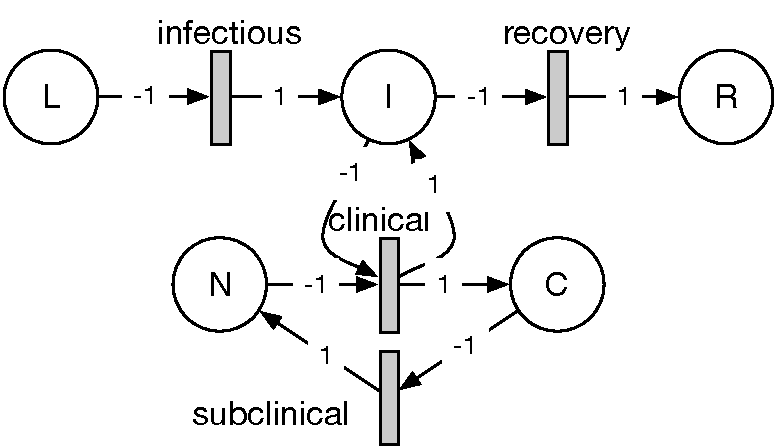
\includegraphics[width=9cm]{individual_gspn}}
\caption{The four compartmental states of an animal with FMDV
are represented by two categories, $(S,I,R)$ and $(N,C)$
where $N$ and $C$ represented not-clinical or clinical.
Computation proceeds by moving a token among $(S,I,R)$ and a
second token among $(N,C)$. Rectangles represent transitions,
which are enabled only when tokens are at all input edges to the
transition.\label{fig:individual_gspn}}
\end{figure}%
In particular, notice that the work of Mardones et al.\ focused
on the most important transition intervals, skipping the $t_3-t_2$
interval in favor of the statistics of the duration of infectious
period. This suggests representation of the two kinds of states,
one for the infectiousness and one for the clinical sign.
Fig.~\ref{fig:individual_gspn} shows these separate systems
and how they are coupled.
Together, these states
represent all of the compartments. An individual can become clinical
only once infectious. As an approximation given the paper's data, the individual
will become subclinical again once recovered.

Note that in Fig.~\ref{fig:compartments} there are two distributions
given for each transition, one exponential and one chosen
to fit the shape of the distribution. Exponential distributions
are often simpler to simulate and are the MaxEnt choice when
only the rate of a transition is known, or when only the rate
of a transition is relevant to predictions from the simulation.
Each version, one with exponential distributions, and one
with non-exponential distributions, will be simulated for
comparison.

Simulations of both models show that, while average rates
are the same, the distribution
of times to infection or recovery can be quite different.
How much this matters depends on the application, which
here is prediction of prevalence within a herd.

\section{Herd Models}
Spread of infection within a herd of cattle is complicated.
Using a compartmental model built from the individual
models above distills complication into variation in
individual compartments and transitions, contact structure,
and infection rate given that contact structure.
How cattle fraternize in a field can be seen as a
time-dependent contact graph whose structure is 
distinct from the infection process which takes place
on that graph. For instance, if the shortest path between
two individuals in the graph is four individuals long, then
\emph{any\/} disease will require two latent periods
to travel from one individual to another.

\begin{itemize}
  \item Exponential or non-exponential individual model.
  \item Time-dependent contact hazard or frequency-dependent contact.
\end{itemize}

\bibliography{cattleherd}
\bibliographystyle{plain}
\end{document}
